\documentclass{article}
\usepackage{graphicx}
\usepackage{amsmath}
\usepackage{tikz}
\title{Reaction-Advection-Diffusion Models of Air Pollution}
\author{Daniel Henricks}


\begin{document}

\maketitle

\section{Introduction}

Airborne pollutants are the single most impactful environmental risk to human health, with about one in nine deaths worldwide
attributed to air pollution (Cohen et al., 2017). Poor air quality can cause many negative implications to human health; exposure to
more air pollution is directly correlated to an increased rate of heart attacks and asthma. There are a few different types of air pollution
that can cause adverse affects on human health. First, fine particulate matter ($\text{PM}_{2.5}$) causes approximately 95\% of the deaths due 
to air pollution. ($\text{PM}_{2.5}$) is defined to be any microscopic particles that are of diameter of less than $2.5 \mu$m, about 20 times smaller than the diameter of
a human hair. 

Due to the minute scale of these particles, particulate matter is capable of traveling deep into vital organs such as the lungs or the bloodstream.
Exposure to increased rates of fine particulate matter can lead to coughing and difficulty breathing. Particulate matter is typically produced by the combustion of gasoline, oil, or wood, but has recently
been discovered to occur at smaller rates from natural processes such as volcanic eruptions (Thangavel et al., 2022). In addition to particulate matter, surface-level ozone
($\text{O}_3$) and nitrogen dioxide ($\text{NO}_2$) also contribute to the damages to human health from air pollution. In this paper, we will validate recent diffusion models of 
air pollution and the models to estimate damages to human health caused by pollution.

\section{Types of Models}

Before beginning on the mathematics behind a differential equation model of air pollution, we will discuss how to form a model of air pollution.
One of the main problems with making a diffusion model for air pollution is estimating the flux term of the diffusion equation. We apply Fick's first and second laws of diffusion; 
recall that Fick's first law relates the flux, $J$ to the diffusion constant $k$, and the change in the concentration gradient $c$:

\begin{equation}
    J = -k \* \frac{dc}{dx}
\end{equation}

Typically, chemical transport models (CTMs), programs that simulate and predict atmospheric chemistry, are used to find the fluxes needed in a diffusion equation. 
There are two classes of CTMs: Eulerian and Lagrangian. Eulerian models have an observer standing in one location who is watching the air pass by, 
whereas the Lagrangian models have the observer moving along with the parcel of air as it takes a random walk through the atmosphere (Vallero, 2021).

However, executing CTMs can be computationally difficult. We will first look at a simple model for representing the concentrations of chemicals in the 
atmosphere.

\section{A Simple Model}

The model we will first investigate is called the one-box model (Jacob, 1999).

\begin{figure}[h]
   \centering
   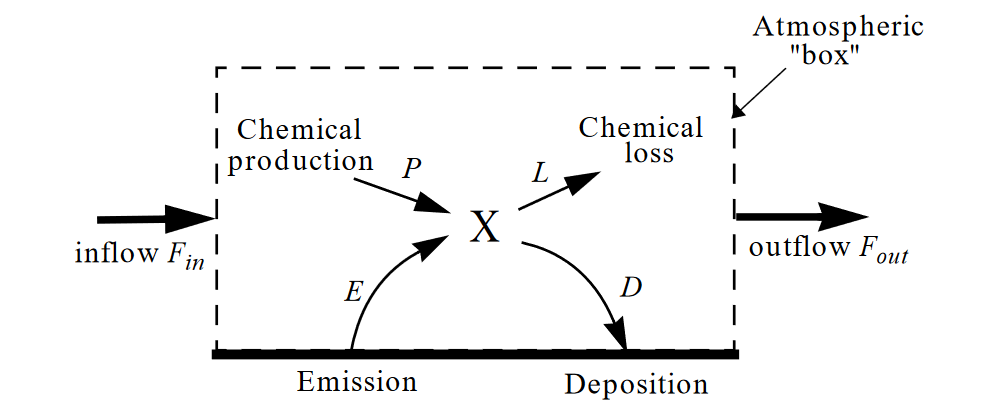
\includegraphics[width=0.8\textwidth]{atmospheric_model.png}
   \caption{One-box model for an atmospheric species X}
   \label{fig:atmospheric_box_model}
\end{figure}

The one-box model for an atmospheric species X is illustrated in Figure~\ref{fig:atmospheric_box_model}. 
The model describes the concentration of X inside of some subset of the global atmosphere (ex: the United States).
The transport rate is described using the flow in, $F_{in}$, and the flow out of, $F_{out}$ of the box. By conservation, the global
atmosphere must obey
$$
    F_{in} = F_{out} = 0
$$
The other parameters of the model are:
\begin{itemize}
   \item Chemical production ($P$)
   \item Emissions ($E$)
   \item Chemical loss ($L$)
   \item Deposition ($D$)
\end{itemize}

We will now define the lifetime, $\tau$, of a molecule, to be the average time a molecule of X remains in our box. 
This will be the mass of the particle divided by the outflow of the box:

\begin{equation}
    \tau = \frac{m}{F_{out}+L+D}    
\end{equation}

\end{document}
